\documentclass{article}
% General document formatting
\usepackage[margin=0.7in]{geometry}
\usepackage[parfill]{parskip}
\usepackage[utf8]{inputenc}
\usepackage{graphicx}
\graphicspath{ {./images/} }

% Related to math
\usepackage{amsmath,amssymb,amsfonts,amsthm}

\title{Homework 1}
\date{9/12/2021}

\begin{document}
\maketitle

\textbf{Name}: Giulio Duregon
\section{Dear Grader}
I've never written proofs before (as you'll soon see), and this is my first time using overleaf. I did my best to demonstrate my conceptual knowledge by elaborating on my answers as much as possible using the English language. If they seem long winded at times, or somewhat amateur in a mathy way, its because I'm still learning how to do this thing. Thanks for your patience!

\break

\section{Problem 1.1 Pictures of E1,E2,E3 can be found on next page}

A set of vectors is a subspace if and only if:
\begin{itemize}
    \item 1) The set of vectors is closed under addition
     \item 2) The set of vectors are closed under scalar multiplication
     \item 3) The set of vectors must include the {0} vector
\end{itemize} 
\par

a)  $x + 5y = 2$ IS NOT a subspace. \par

The following equation: $x + 5y = 2$, is a line in $\mathbb{R}^2$ that does not pass through the origin. As it does not pass through the origin, the set does not contain the zero vector, and therefore is not a subspace. For example, try entering $x=0,y=0$ into our equation $x+5*y=2$ which gives us: $0+(5*0)=2$ which of course does not hold.
\par
b) Yes, $x +5y = 0$ IS a subspace, with $Dim(\mathbf{E}_2)=1$, with basis vector
$\begin{pmatrix}
5\\
-1
\end{pmatrix}$
\par
You can rewrite   $x +5y = 0$ as $x = -5y$ which is a line passing through the origin in $\mathbb{R}^2$. It is a subspace because:

\begin{itemize}
    \item We know that our line is closed under multiplication as multiplying our vector by any scalar simply moves it along it's own span
    \subitem $\alpha(x+5y) = \alpha x + \alpha 5y = 0 \Longleftrightarrow \alpha x = -\alpha 5y$
    \item Our line is closed under addition, as we can add any two arbitrary vectors from our subspace together and remain in our line: 
    \subitem $(x+5y) + (2x+10y) = 3x + 15y = 0 \Longleftrightarrow 3x = -15y \Longleftrightarrow x=-5y$
    \item Our line crosses through the origin, and therefore includes the 0 vector. 
    \subitem Take $x=0,y=0$ and  $0+(5*0)=0$
\end{itemize}


c) $x^2$ + $y^2$ = 2 IS NOT a subspace. \par
The equation $x^2$ + $y^2$ = 2 inscribes a circle with radius = $\sqrt{2}$ around the origin. We can quickly conclude that this is not closed under addition by adding vectors with terms that satisfy the equation. \par
Take two (x,y) pairs, say ($\sqrt{2}$,0) and (0,$\sqrt{2}$), both which are in $\mathbf{E}_3$ (the (x,y) pairs satisfy $x^2 + y^2 = 2$). \par
If you try adding the two pairs together ($\sqrt{2}$,0) + (0,$\sqrt{2}$) = ($\sqrt{2}$,$\sqrt{2}$) which is not in $\mathbf{E}_3$ ($\sqrt{2}^2$ + $\sqrt{2}^2 = 4 \neq 2$ and therefore does not satisfy $x^2 + y^2 = 2$ ). \par
Hence, it has been proved that $\mathbf{E}_3$ is NOT closed under addition, and therefore, is not a subspace of $\mathbb{R}^2$. Also, it does not include the 0 vector (by definition of $x^2 +y^2=2$), and therefore is not a subspace.

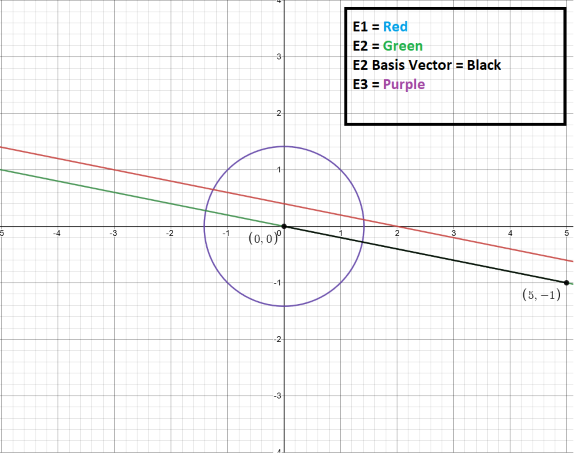
\includegraphics{Figure1.png}

\break

\section{Problem 1.2}

Again, a set of vectors is a subspace if and only if:
\begin{itemize}
    \item 1) The set of vectors is closed under addition
     \item 2) The set of vectors are closed under scalar multiplication
     \item 3) The set of vectors must include the {0} vector
\end{itemize} 

a) $\mathbf{E}_4$ defined by $x+y=0$ is a subspace of $\mathbb{R}^3$ with $Dim(\mathbf{E}_4)=1$ with basis: $\begin{pmatrix}
1\\
-1\\
0
\end{pmatrix}$ 
\par
To intuitively understand why, $x+y=0$ can be rewritten as $x = -y$, and understood as a one-dimensional line crossing through the origin in ${R}^3$ space.
\begin{itemize}
    \item We know that our line is closed under multiplication as multiplying our vector by any scalar simply moves it along it's own span
    \subitem $\alpha(x+y) = \alpha x + \alpha y = 0 \Longleftrightarrow \alpha x = -\alpha y$
    \item Our line is closed under addition, as we can add any two arbitrary vectors from our subspace together and remain in our line: 
    \subitem $(x+y) + (2x+2y) = 3x + 3y = 0 \Longleftrightarrow 3x = -3y \Longleftrightarrow x=-y$
    \item Our line crosses through the origin, and therefore includes the 0 vector. 
    \subitem Take $x=0,y=0$ and  $0+0=0$
\end{itemize}

\par

b) $\{x+y=0$ , $-y+3z=0\}$ is a subspace of $\mathbb{R}^3$, it is a hyper-plane with dimension $Dim(\mathbf{E}_5)=2$ and basis $\begin{pmatrix}
1 , 0\\
-1 , 1\\
0 , 3
\end{pmatrix}$
\\
\par
We can understand $x+y=0$ as a line through the origin defined by $x=-y$. Likewise we can understand $-y+3z =0$ as a line through the origin defined by $y=3z$. The span of these two vectors is any linear combination of the two (hence the aforementioned basis and dimension). We already proved that lines that pass through the origin are:
\begin{itemize}
    \item Closed under multiplication
    \item Closed under addition
    \item Includes the origin
\end{itemize}
Which can be applied to our new line $-y+3z =0$. Any linear combination of our two lines will hold these properties, and remain a subspace.
\par


\break

\section{Problem 1.3}
a) The family of vectors $e = (e_1, \dots, e_n)$ is a basis of ${R}^n$ with $Dim(e)=n$, as, by definition:
\begin{itemize}
    \item All the vectors in $e_1,\dots,e_n$ are linearly independent (no linear combination of vectors can form another vector in the basis). For example, lets consider $\mathbb{R}^2$. We have $e_1 = (1,0)$ and $e_2 = (0,1)$. We cannot multiply $e_1$ by any scalar to create $e_2$. Likewise, we cannot multiply $e_2$ by any scalar to create $e_1$. This holds for all of $e$ in any $\mathbb{R}^n$
    \item The vectors in $e_1,\dots,e_n$ span all of ${R}^n$ (a linear combination of the basis vectors can be made to reach any point in $\mathbb{R}^n$). Lets consider $\mathbb{R}^2$, where we have basis vectors $e_1 = (1,0)$ and $e_2 = (0,1)$. We can reach any point in $\mathbb{R}^2$ space with linear combinations of our basis vectors. If we wanted to reach the arbitrary point (x,y), we could scale $e_1$ by $x$ and $e_2$ by $y$. The linear combination would result in: $x(1,0)+y(0,1) = (x,0)+(0,y) = (x,y)$
\end{itemize}\par

b) 
\begin{itemize}
    \item Example of a hyper-plane in ${R}^n$ for a subset of the family of $e = (e_1, \dots, e_n)$ vectors would be: $e = (e_1, \dots, e_{n-1})$, as in a set of $n-1$ vectors with $Dim(Hyper-Plane) = n-1$. If we wanted an example in $\mathbb{R}^3$ then our basis would be \{$e_1,e_2$\}  and our hyper-plane would $Span(e_1,e_2)$ and have $Dim(e_1,e_2)=2$
    \item Example of a line in ${R}^n$ for a subset of vectors for the family of  $e = (e_1, \dots, e_n)$ would be $e = (e_1)$, as in the set of vectors that includes ONLY one vector with basis \{$e_1$\} and $Dim(e_1) = 1$
\end{itemize}
\break

\section{Problem 1.4}

    a) Assume the family of vectors $v = {v_1,\dots, v_q}$ in $\mathbb{R}^n$ has more than n vectors. 
    \par
    If that is the case, there is some linear combination of vectors within $v = {v_1,\dots, v_q}$ that can make up at least one vector in $v = {v_1,\dots, v_q}$. That would mean the family $v = {v_1,\dots, v_q}$ is LINEARLY DEPENDANT.\par
    However, it is stated that the family of vectors is LINEARLY INDEPENDENT, therefore, it must have $q\leq n$ vectors. If we knew that the family of vectors $v$ spanned all of $\mathbb{R}^n$ then we would know for certain it contains $n$ vectors. As we don't know this for certain, we know that it has up to $n$ vectors.

\par
b) Assume that there are less than $n$ vectors in the family of vectors $u = {u_1, \dots, u_p}$, say $p=n-1$ for example. 
\par
If that is the case, at most the span of $u = {u_1, \dots, u_p}$ resembles a hyper plane in $\mathbb{R}^n$ as $Dim(u)=n-1$ (recall that hyper-planes are defined as $dim()=n-1$), and therefore, does not span all of $\mathbb{R}^n$.
\par
However, we know that the family of vectors $u = {u_1, \dots, u_p}$ spans all of $\mathbb{R}^n$, and therefore, we know that $p\geq n$. In essence, since the family $u$ spans all of $\mathbb{R}^n$ it must have at least n vectors, but it could have many more, as it is not given that it is a linearly independent set.

\par
c) Here's what we have:
\begin{itemize}
    \item a linearly independent set of vectors $v = {v_1,\dots, v_q}$ that do not span all of $\mathbb{R}^n$ (Where $q<n$)
    \item a linearly dependant family of vectors $u = {u_1, \dots, u_p}$ that does span all of $\mathbb{R}^n$ (Where $p\geq n$)
\end{itemize}
Lets make a new set of vectors that includes all the vectors of $v$ and add to them the necessary number of vectors from $u$ to span all of $\mathbb{R}^n$ while still having our set be linearly independent. If we have $q$ vectors from $v$ and $m-q$ vectors from $u$ we have $q+(m-q)=m$ vectors. Since our new set of vectors spans all of $\mathbb{R}^n$, and is linearly independent, our set of vectors is a basis for $\mathbb{R}^n$. We know by Theorem 3.2 that if any vector space V admits a basis $(v_1,\dots,v_n)$, then every basis of V will have n vectors. Therefore, $m=n$.
\par

d) Using vectors in the set $u = (u_1, \dots, u_5)$ and vectors $e_1 = (1,0,0,0)$ and $e_3 = (0,0,1,0)$ we can construct a basis for $\mathbb{R}^4$. Specifically, we will use the vectors $u_3 = (1,0,0,1)$ and $u_5 = (0,1,1,0)$ as we can get $e_2 = (0,1,0,0)$ and $e_4 = (0,0,0,1)$ from using linear combinations of the vectors. 

\begin{itemize}
    \item $e_2 = u_5 - e_3$ also expressed as  $(0,1,1,0)-(0,0,1,0) = (0,1,0,0) = e_2$   
    \item $e_4 = u_3 - e_1$ also expressed as  $(1,0,0,1)-(1,0,0,0) = (0,0,0,1) = e_4$  
\end{itemize}
We have proved that we can form a basis for $\mathbb{R}^4$ using the the set of vectors $\{e_1,e_3,u_3,u_5\}$, as a linear combination of those vectors can form the canonical basis $\{e_1,e_2,e_3,e_4\}$ (which of course, spans all of $\mathbb{R}^4$ and is linearly independent).

\break
\section{Problem 1.5}
We have V and G, two vector spaces of finite dimension. We must prove the equivalence of the following two statements:
\begin{itemize}
    \item $V=G$ $\Longleftrightarrow$ $Dim(V) = Dim(G)$ and $V\subset G$ 
\end{itemize}
If V and G are equal they must have the same dimension, as well as the same span. If these two conditions are met,  every element of V will be in G, and every element in G will be in V. 
\par
However, if we are only given one statement at a time, we cannot prove their equivalence. Allow me to demonstrate:
\begin{itemize}
    \item Firstly, consider V and G each have one vector as their basis. Say $Basis(G) = (1,1)$ and $Basis(V)=(1,-1)$. Both vector spaces would be lines in $\mathbb{R}^2$, and $Dim(G)=1$ and $Dim(V)=1$. Their dimension would be equal, but the lines are linearly independent with completely different spans. No element (other than the 0 vector) would be shared between the two vector spaces, and therefore they are not equivalent.
    
    \item Secondly, assume we only know the fact that V is a subset of G. Consider the following basis for our vectors spaces V and G, each in $\mathbb{R}^3$: $Basis(V)=\{(1,0,0)$ and $(0,1,0)\}$ and $Basis(G)=\{(1,0,0)$ and $(0,1,0)$ and $(0,0,1)$\}. Here we can clearly see that every possible element in V can be found in G, as they each share the basis vectors $(1,0,0)$ and $(0,1,0)$, and therefore can make any linear combination of the two vectors (re: Span). However, as $Dim(Span(V))=2$ and $Dim(Span(G))=3$ we know that there are elements of G that cannot be found in V (The third vector in G $(0,0,1)$ allows G to have greater span).
  
\end{itemize}
\par
Again, consider the first example, where $Dim(V)=Dim(G)=1$ and their spans were each a line in $\mathbb{R}^2$. If we are given the fact that $V\subset G$, then the two vector spaces must share the same span. IF they share the same span, and have the same dimension, then $V=G$.\par
Likewise, this can be proved the other way around: if we start  with $V\subset G$, we have our example outlined in my second bullet point. However, if we find out that $Dim(V) = Dim(G)$, it rules out the possibility of G having a span greater than Vs. If they have the same dimension, and all elements of V are in G, it follows that all elements in G are in V. Hopefully this was clear :)




\break
\section{Graphics for Problem 1.1}
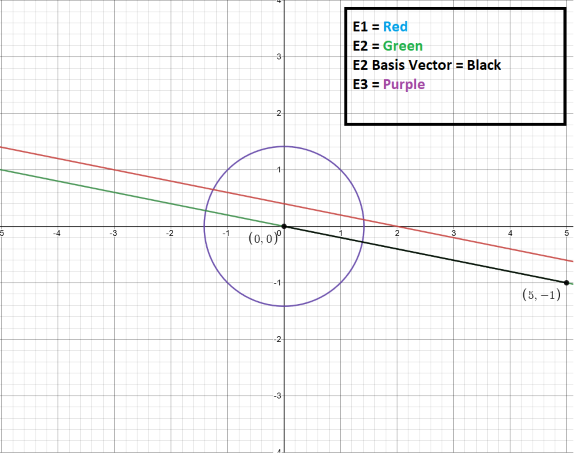
\includegraphics{Figure1.png}
\end{document}